\documentclass{article}
\usepackage{listings}
\usepackage{pdfpages}
\usepackage{graphicx}
\begin{document}
\title{Modelos y Optimizaci\'on I\\ \large{Trabajo pr\'actico: Problema Combinatorio}}
\author{de Valais, Ezequiel (94463)\and	Rozanec, Matias (97404)}
\date{Octubre 2017}
\maketitle
\newpage
% FIN PRESENTACION

% Indice
\tableofcontents
\newpage

% Consigna
%\part{Consigna}
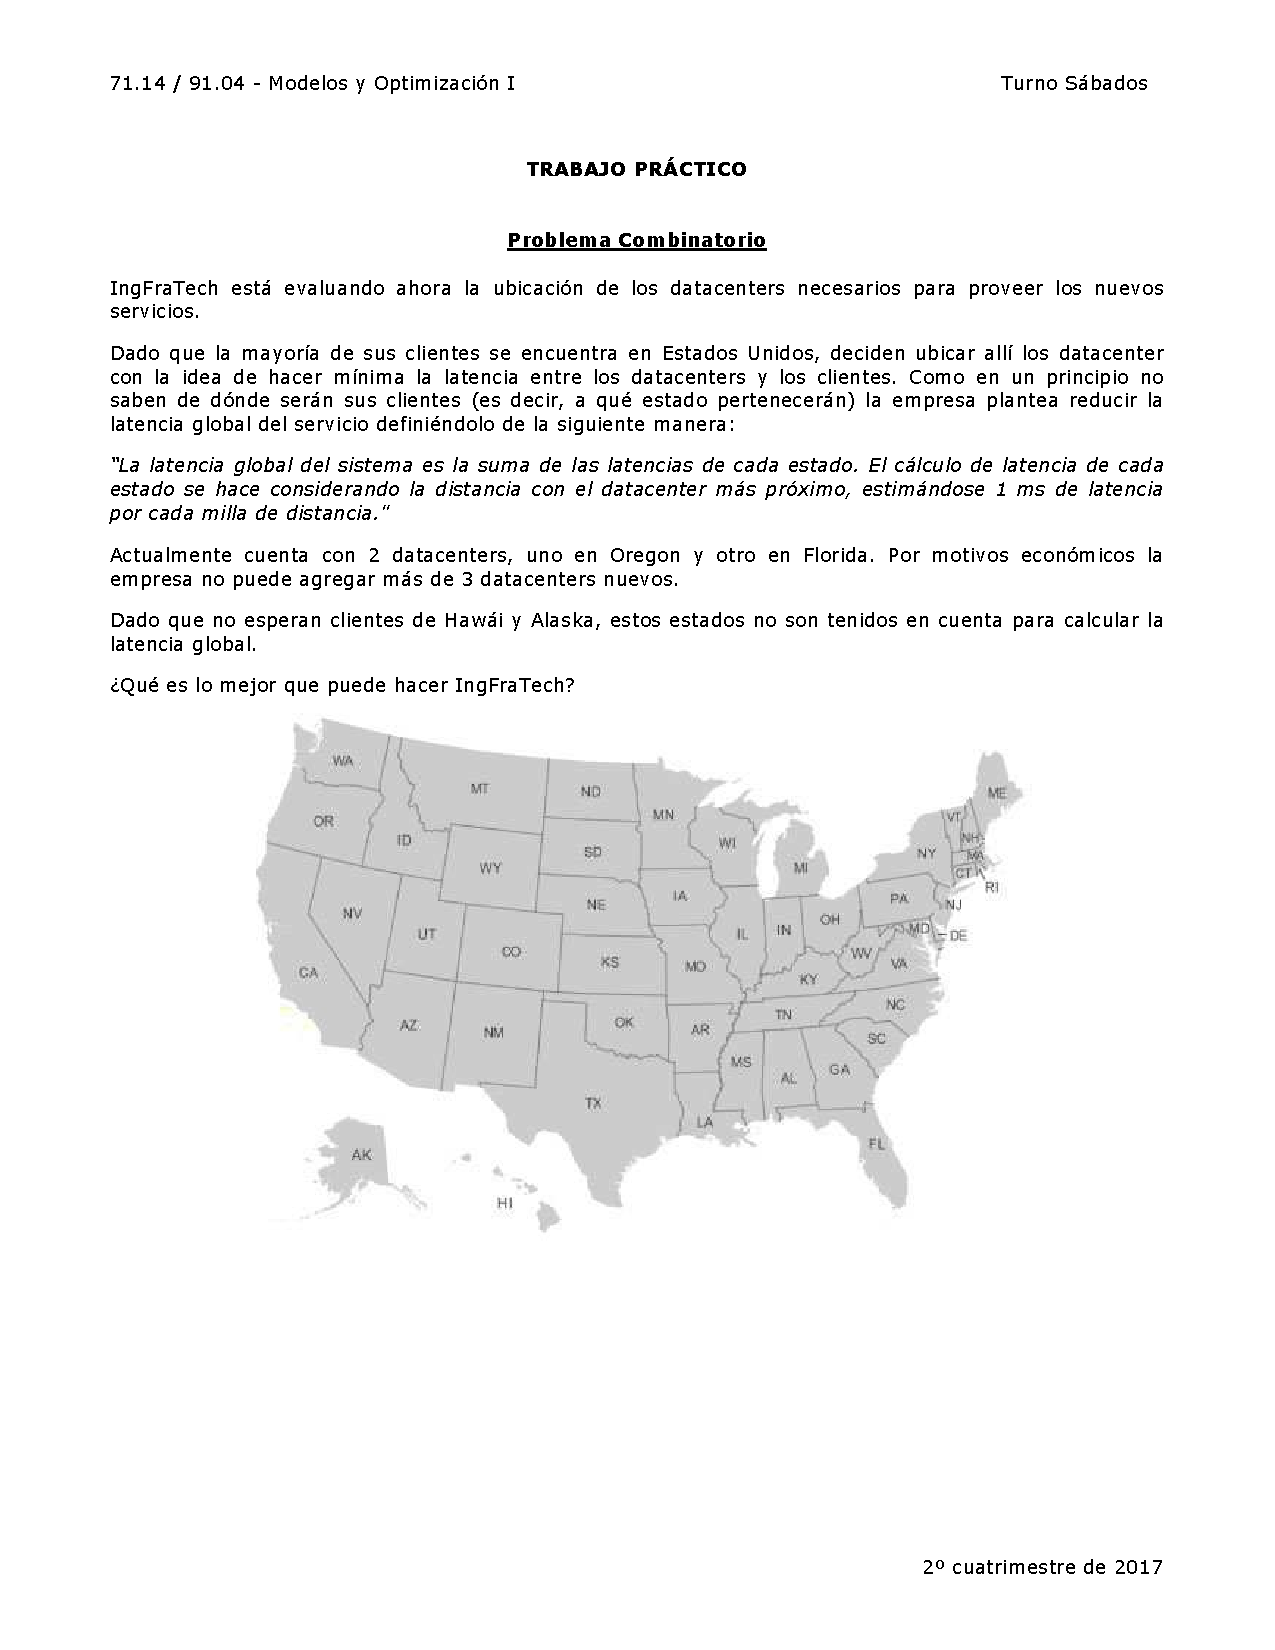
\includepdf{EnunciadoProblemaCombinatorio.pdf}
\newpage

% Resolucion

% Intro
\part{Descripci\'on de la situaci\'on problem\'atica}
Se trata de un problema de combinatoria, en el que habr\'a que incluir variables continuas y booleanas. \\
En esta instancia podemos afirmar que habr\'a que considerar una variable \textit{latencia} que deber\'a ser una variable continua; as\'i como una variable booleana que indique si un determinado datacenter se encuentra instalado en un estado espec\'ifico.

% Objetivo
\part{Objetivo}
Determinar en qu\'e estados van a estar los 3 nuevos datacenters ($DB, DC, DD$) durante un per\'iodo de tiempo para minimizar la latencia global del sistema.

% Hipotesis
\part{Hip\'otesis y supuestos}
\begin{itemize}
	\item Se instalar\'an los 3 datacenters puesto que cada datacenter agregado va a reducir la latencia.
	\item Se tomar\'a un punto en cada estado. El mismo ser\'a referente para calcular las distancias entre estados y las respectivas latencias. No hay opci\'on de instalar un datacenter en otro punto del estado que el mencionado.
	\item Para el c\'alculo se consideran \'unicamente las distancias, no la cantidad de usuarios por estado. O expresado de otra forma: para el modelo, la distribuci\'on de usuarios es uniforme a lo largo de todos los estados y en cada uno de los estados. 
	\item No puede haber dos datacenters en un mismo estado.
	\item Los costos de instalaci\'on y mantenimiento de datacenters, as\'i como cualquier otro costo que pueda implicar la instalaci\'on de los mismos, no ser\'an tenidos en cuenta por el modelo.
\end{itemize}
\newpage

% Variables
\part{Definici\'on de variables, incluyendo unidades}
\begin{itemize}
	\item $L_{i}$ : variable continua que indica la latencia (en ms) correspondiente al estado i. $\forall i \in [1, 48]$
	\item $DC_{i}$ : variable continua que indica la distancia (en millas) del datacenter $C$ al estado $i$. (\'idem para datacenters $D$ y $E$. $DA_{i}$ y  $DB_{i}$ son datos conocidos). $\forall i \in [1, 48]$
	\item $YA_{i}$ : variable bivalente que vale 0 cuando el estado $i$ tiene la menor latencia. (\'idem $B,C,D,E$)
	\item $YCe_{i}$ : variable bivalente que vale 1 cuando el datacenter $C$ est\'a en el Estado $i$. (\'idem $D, E$)
\end{itemize}
% Constantes
\section*{Constantes}
\begin{itemize}
\item $D_{ij}$: distancia entre estado $i$ y estado $j$.
\item $M$: valor mayor a cualquier distancia posible. Su valor se definir\'a al momento de pasar el modelo a software.
\end{itemize}

\part{Modelo de Programaci\'on Lineal Continua}

\begin{equation}
	\sum_{i} YA{i} + YB_{i} + YC_i + YD_i + YE_i = 1
\end{equation}

\section{Menor Distancia}
Cada $L_i$ tendr\'a como cota superior la distancia al datacenter m\'as pr\'oximo, y como cota inferior esa misma distancia en el caso de que el estado $i$ tenga la menor distancia.\\
$M \rightarrow \infty$
\begin{equation}
DA_{i} - M * YA_{i} \leq L_{i} \leq DA_{i}, \quad \forall i \in [1, 48]
\end{equation}
\begin{equation}
DB_{i} - M * YB_{i} \leq L_{i} \leq DB_{i}, \quad \forall i \in [1, 48]
\end{equation}
\begin{equation}
DC_{i} - M * YC_{i} \leq L_{i} \leq DC_{i}, \quad \forall i \in [1, 48]
\end{equation}
\begin{equation}
DD_{i} - M * YD_{i} \leq L_{i} \leq DD_{i}, \quad \forall i \in [1, 48]
\end{equation}
\begin{equation}
DE_{i} - M * YE_{i} \leq L_{i} \leq DE_{i}, \quad \forall i \in [1, 48]
\end{equation}

\section{Asociaci\'on de Datacenter a estado}
Se asegura de que cada datacenter pueda ser asignado \'unicamente a un estado.
\begin{equation}
\sum_{i=1}^{48} YCe_{i}  = 1
\end{equation}
\begin{equation}
\sum_{i=1}^{48} YDe_{i}  = 1
\end{equation}
\begin{equation}
\sum_{i=1}^{48} YEe_{i}  = 1
\end{equation}

\section{Asociaci\'on de distancia de un estado al datacenter correspondiente}
\begin{equation}
DC_{i} = 
\sum_{j=1}^{48} D_{ij} * YCe_{j}          
\end{equation}
\begin{equation}
DD_{i} = 
\sum_{j=1}^{48} D_{ij} * YDe_{j}          
\end{equation}
\begin{equation}
DE_{i} = 
\sum_{j=1}^{48} D_{ij} * YEe_{j}, \quad \forall i \in [1, 48]
\end{equation}

\part{Funcional}
\begin{equation}
Z(min) =
\sum_{i=1}^{48} L_{i} 
\end{equation}

\newpage
% modelo y salida
\part{Modelo y salida}

\
\lstset { %
	language=C++,
	backgroundcolor=\color{black!5}, % set backgroundcolor
	basicstyle=\footnotesize,% basic font setting
	linewidth=14cm,
	showstringspaces=true,
	numbers=left,
	numberstyle=\tiny,
	breaklines=true,
	tabsize=4,
}
\lstinputlisting[frame=single]{modelo/comb.mod}

\newpage

\
\lstset { %
	language=C++,
	backgroundcolor=\color{black!5}, % set backgroundcolor
	basicstyle=\footnotesize,% basic font setting
	linewidth=14cm,
	showstringspaces=true,
	numbers=left,
	numberstyle=\tiny,
	breaklines=true,
	tabsize=4,
}
\lstinputlisting[frame=single]{modelo/comb.sol}

\newpage
% Conclusiones
\part{Conclusiones}

Se decidi\'o realizar la corrida sobre los siguientes estados:
\smallskip\\
Alabama, Arizona, Arkansas, California, Colorado, Connecticut, Florida, Oregon
\bigskip\\
Fuera de Florida (Datacenter A) y Oregon (Datacenter B), las 3 nuevas datacenters son las siguientes
\bigskip\\
Datacenter C: Colorado        (77 YCei[Colorado]      1)
\smallskip\\
Datacenter D: Arkansas        (83 YDei[Arkansas]      1)     	
\smallskip\\
Datacenter E: Connecticut     (94 YEei[Connecticut]   1)   
\bigskip\\
La latencia global del sistema es: 1457.681632
\bigskip\\
Las latencias de cada estado son las siguientes:
\bigskip\\
Li[Alabama]       223.749        
\smallskip\\     
Li[Arizona]       817.982       
\smallskip\\      
Li[Arkansas]      0            
\smallskip\\ 
Li[California]    415.951     
\smallskip\\  
Li[Colorado]      0         
\smallskip\\    
Li[Connecticut]   0     
\smallskip\\        
Li[Florida]       0   
\smallskip\\          
Li[Oregon]        0             
\bigskip\\
Esto tiene sentido pues solo Alabama, Arizona y California no tienen un datacenter en el estado.
\bigskip\\
El datacenter C de Colorado es el mas cercano a Arizona (la distancia del datacenter al estado es la misma que su latencia m\'inima):
\smallskip\\
DCi[Arizona]          817.982 
\bigskip\\
El datacenter A de Florida es el mas cercano a Alabama (define la cota inferior a la latencia del estado) 
\smallskip\\
cota_inf_dcA[Alabama]   223.749  
\bigskip\\
El datacenter B de Oregon es el mas cercano a California (define la cota inferior a la latencia del estado) 
\smallskip\\
cota_inf_dcB[California] 415.951 
\bigskip\\


\newpage
% HEURISTICA
\part{Heur\'istica}
\begin{verbatim}
compilar: g++ -std=c++11 heuristic.cpp -o heuristic
correr: cat distances.csv  | ./heuristic
\end{verbatim}

\
\lstset { %
	language=C++,
	backgroundcolor=\color{black!5}, % set backgroundcolor
	basicstyle=\footnotesize,% basic font setting
	linewidth=14cm,
	showstringspaces=true,
	numbers=left,
	numberstyle=\tiny,
	breaklines=true,
	tabsize=4,
}
\lstinputlisting[frame=single]{Heuristica/heuristic.cpp}





\newpage
% Conclusiones Heur\'istica
\part{Resultados de Heur\'istica}

Se corri\'o la heur\'istica con los 8 estados y se consiguieron los siguientes resultados:
\begin{verbatim}
Insert number of state where datacenter 1 should be.
latency after datacenter 1 was allocated: 16236.8
Insert number of state where datacenter 2 should be.
latency after datacenter 2 was allocated: 6209.89
latency after datacenter 3 located: 4902.32
latency after datacenter 4 located: 2353.21
latency after datacenter 5 located: 1937.26
*** Final datacenter positions ****
datacenter	1	located in state	7
datacenter	2	located in state	8
datacenter	3	located in state	6
datacenter	4	located in state	5
datacenter	5	located in state	4
\end{verbatim}

\smallskip\\
Los datacenters seleccionador quedaron en los estados California Colorado y Conetticut (4, 5 y 6) dejando la latencia en 1937.26
\smallskip\\
Este resultado es peor comparado con el modelo de GLPK que dej\'o la latencia en 1457
\bigskip\\


Se corri\'o la heur\'istica con los 48 estados y se consiguieron los siguientes resultados:
\begin{verbatim}
Insert number of state where datacenter 1 should be.
latency after datacenter 1 was allocated: 68827.2
Insert number of state where datacenter 2 should be.
latency after datacenter 2 was allocated: 44071.9
latency after datacenter 3 located: 32303.7
latency after datacenter 4 located: 27360.3
latency after datacenter 5 located: 22764.1
*** Final datacenter positions ****
datacenter	1	located in state	8
datacenter	2	located in state	35
datacenter	3	located in state	48
datacenter	4	located in state	47
datacenter	5	located in state	46

\end{verbatim}
\smallskip\\
Los datacenters seleccionador quedaron en los estados Wyoming, Wisconsin y west virginia dejando la latencia en 22764.1


\end{document}
